\documentclass[11pt,a4paper,article,oneside]{memoir}
% \setulmarginsandblock{3.5cm}{3.5cm}{*}
% \setlrmarginsandblock{3.5cm}{3.5cm}{*}
\usepackage[T1]{fontenc}
\usepackage{lmodern}
\usepackage[english]{babel}
\usepackage[utf8]{inputenc}
\usepackage{microtype}
\setlength{\parskip}{6pt}
\setlength{\parindent}{0pt}

\usepackage{minibox}
\usepackage{listings}
\usepackage{tabu}
\usepackage[hidelinks]{hyperref}
\usepackage{amsmath, amsthm, amssymb}
\usepackage{float}

\usepackage{graphicx}

% \usepackage{wrapfig}
% \usepackage{bchart}
% \usepackage{wasysym}

% \makeoddhead{plain}{\theauthor~- Grupp 4}{}{}
% \makeevenhead{plain}{\theauthor~- Grupp 4}{}{}
% \makeoddfoot{plain}{}{}{}
% \makeevenfoot{plain}{}{}{}

% \usepackage{titlesec}
% \titleformat*{\section}{\large\bfseries}
% \titlespacing\section{0pt}{12pt plus 4pt minus 2pt}{0pt plus 2pt minus 2pt}

% \usepackage[backend=biber]{biblatex}
% \bibliography{bib.bib}

\title{Project prototype implementation}
% \date{}
\author{Konrad Magnusson, Tim Olsson, Alex Sundström, Victor Ähdel}

\checkandfixthelayout{}
\begin{document}
% \begin{titlingpage}
\maketitle
% \end{titlingpage}

\chapter{First implementation}
The base of our particle rendering is still the \verb|glutSolidSphere| provided for us in the OpenGL lab GLFW version. 
However the initialization of the vertices and indices as well as their deletion only happens once instead of every frame. 
Furthermore we also use instanced rendering.
To do this we created another buffer (VBO) to our vertex array object (VAO). 
This second buffer holds floats for the particles position and bytes indicating their type (iron or silicate). 
This buffer is \verb|(4 * GL_FLOAT + GL_BYTE) * NR_PARTICLES| long. 
With \verb|glVertexAttribPointer| and \verb|glVertexAttribDivisor| we can set that this buffer will be used for instanced rendering with a certain stride. 

We also have a very smooth camera that can move around the space very naturally, like a space ship.
The rendering parts are not yet decoupled from the CUDA parts, so if the particle velocity updates are slow the camera suffers though.
But at semi-high frame rates it works incredibly well.

The initialization of the planets are implemented fully.
We had also implemented the angular velocity of the planets before the news that we could use a simplified version, so that should be sufficiently complex.

We have moved our particle updates to CUDA.
Currently, one thread is run for each particle, calculating its change in velocity by iterating through each other particle.
We thus do not yet follow the guidelines set by the Nvidia gems article, but we have a separate \verb|__device__| function for the force calculation, so changing the order of which we compute the ``2d matrix'' will be easy.


\chapter{Initial results}
Due to the instanced rendering the rendering can handle 100 thousand particles at like 30 frames per second.
And that is with spheres with a lot of polygons, we could simplify that and then we would be all set for even more particles.

By using CUDA for the particle velocity updates, we can handle around 3000 particles at 30 frames per second.
We are not quite happy with that, and would like to improve upon it further; see the next chapter.

The ``planets'' stick together somewhat at least, but there are too few particles for gravity to make them truly act like planets.
They are very volatile though, something about the interaction when they collide often make a lot of the iron particles shoot out.

The figures below show the program at some steps in a simulation with a few particles, with parameters modified such that they stick together somewhat well.

\begin{figure}[h]
\center
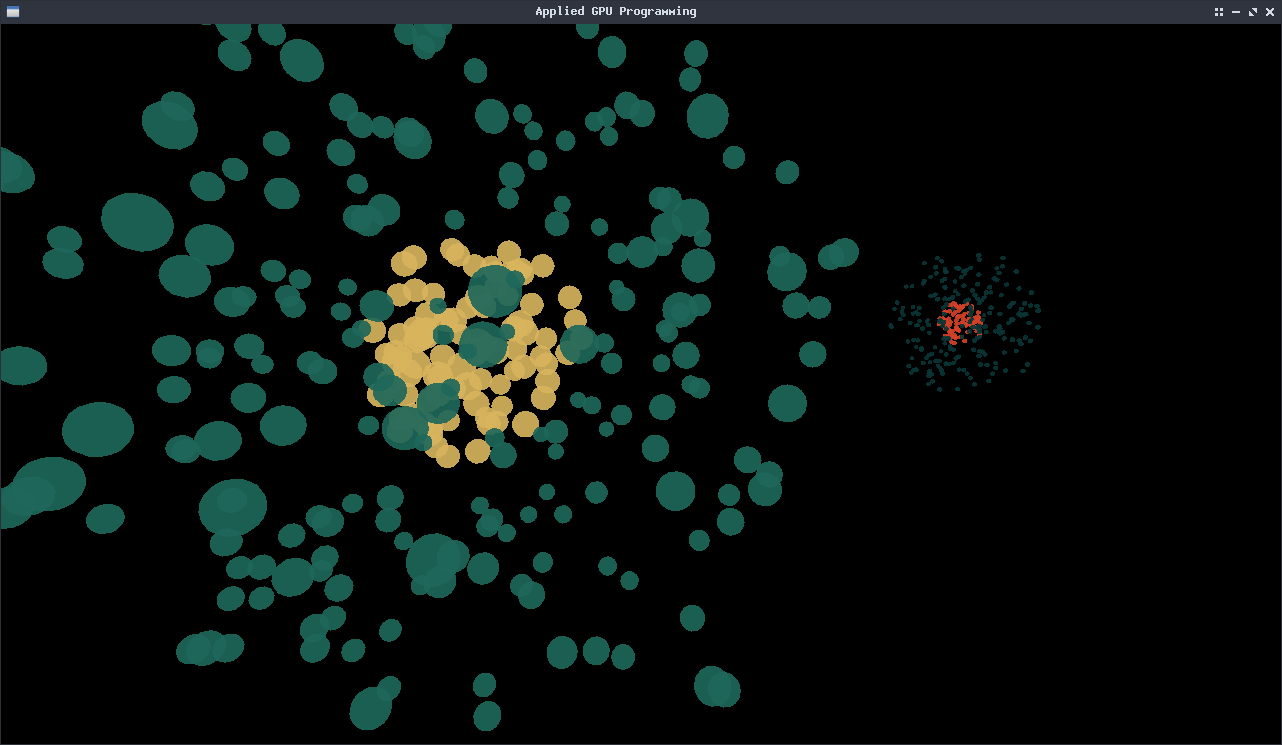
\includegraphics[width=12cm]{img1}
\caption{Start position of two planets}
\end{figure}

\begin{figure}[h]
\center
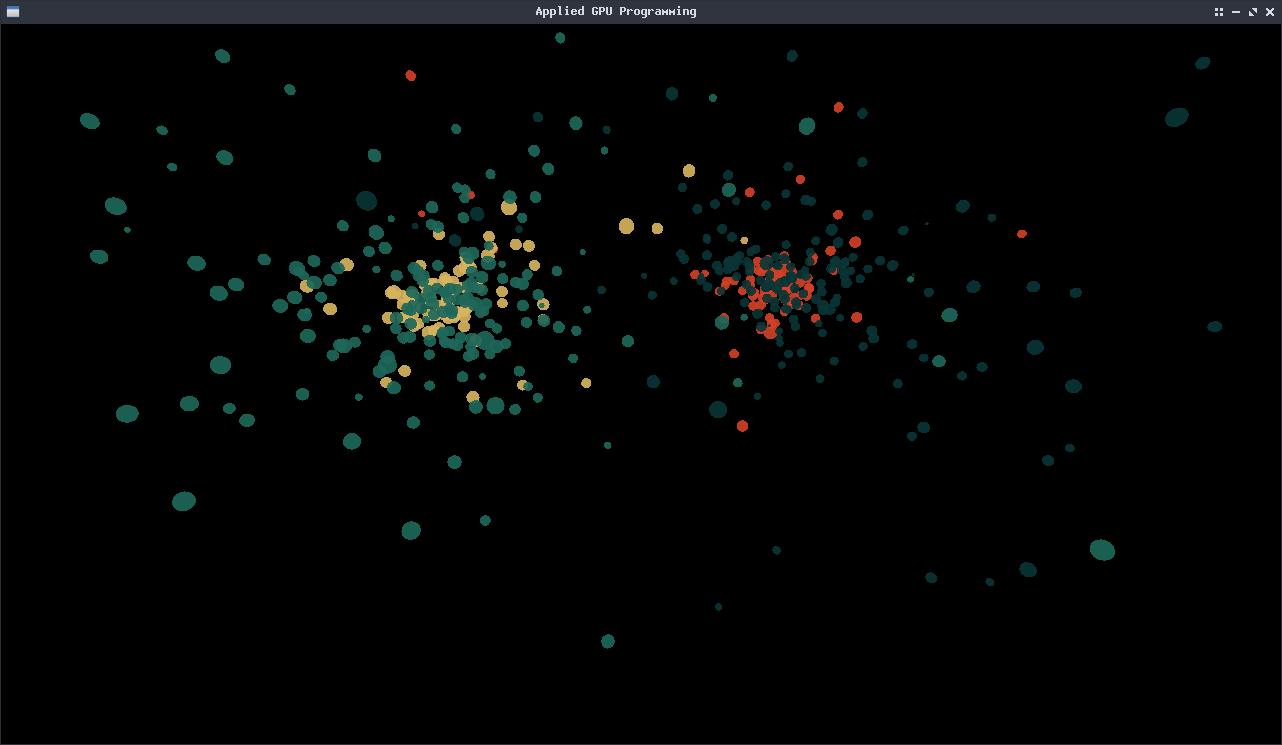
\includegraphics[width=12cm]{img2}
\caption{State after a bit of simulation}
\end{figure}

\begin{figure}[h]
\center
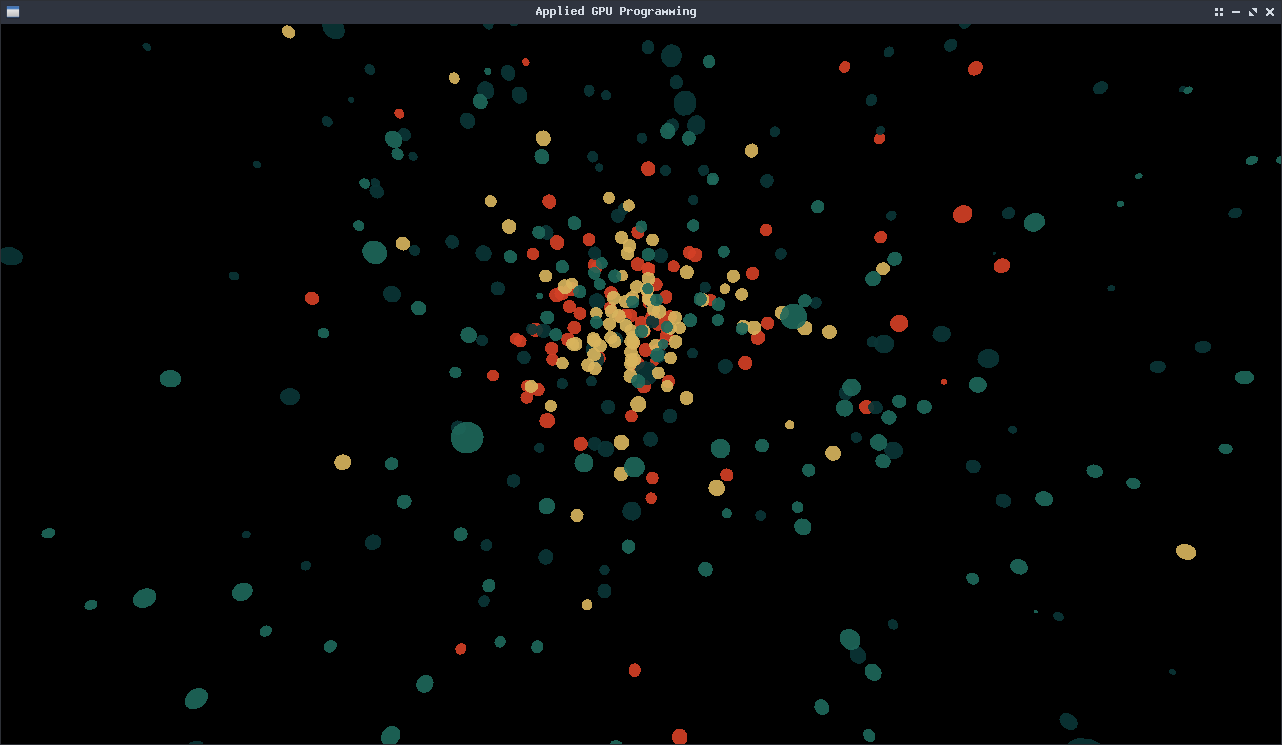
\includegraphics[width=12cm]{img3}
\caption{State after a longer bit of simulation, after the planets have merged}
\end{figure}

\chapter{Next steps}
The OpenGL parts are very much workable, so not much more has to be done there.
Aside from slight optimizations such as using fewer polygons, it is pretty much complete.

We would like to add an FPS- or time-for-last-frame-counter to more easily see the frame-rate.
For that we need to add some text capabilities, since we do not otherwise use any text, so we need some font support.
Other than that we would also like to use some profiler such as \verb|nvprof| or the visual profiler, to further see which parts are slow and could be improved.

The CUDA part needs some improvements, as it is not yet at a speed that we are happy with.
We expect significant improvements by following the steps in the Nvidia gems article, to enable using some shared memory.

Furthermore, we want to change the numerical integration of the forces, possibly using runge-kutta.
This might improve the stability of the planets.

Then we need to enable interop between CUDA and OpenGL.
We have done the previous steps in such a manner that it should not be very difficult, but we need to modify things slightly to write it directly from CUDA.

% \printbibliography{}

\end{document}
